\mychapter{ فصل اول:  زمینه ها و مفاهیم}

\subsection*{مدخل}
\addcontentsline{toc}{subsection}{مدخل}
در این فصل، که در سه گفتار تنظیم گردیده، سعی شده است، مفاهیم پایه و زمینه‌های تاثیر‌گذاری و تاثیر‌پذیری انسان و  محیط‌زیست، معرفی و بیان شود. 
در ابتدا به طرح مسئله از نگاه زمین شناسان پرداخته و آغاز تغییرات گسترده در زمین و مبنای تغییرات‌اقلیمی مورد موشکافی قرار گرفته است. هدف از این گفتار، آشنایی با ویژگی‌های دور جدید زمین‌شناسی است، که به دورانسان\LTRfootnote{Anthropocene}
 معروف گردیده و با ویژگی عدم پایداری مورد شناسایی قرار می‌گیرد. این گفتار به ما در فهم گستردگی، زمینه‌ها و علل بروز تغییرات زیستی کمک می‌نماید. 
در گفتار بعدی به تشریح تغییرات‌اقلیمی، و آثار آن بر نظام اقلیم و جوامع انسانی پرداخته‌ایم. مسیرهای پیشگیری و انطباق با تغییرات‌اقلیمی، ضرورت شناخت علمی این تغییرات را توجیه می‌نماید. در بررسی آثار این تغییرات سعی گردیده از گزارش‌های هیات بین‌الدولی تغییرات‌اقلیمی به عنوان منبع اصلی استفاده شود. 
در گفتار پایانی فصل، حق بر آینده سبز به لحاظ مفهومی تشریح و تبیین شده است. این مفهوم، به طور ضمنی به حقوق کودکان و نسل‌های آینده در گستره زمان اشاره دارد. به همین جهت پس از تبیین حق بر آینده سبز، مفاهیم کودک و نسل‌های آینده به عنوان گروه‌های آسیب پذیر، تعریف گردیده است.



\section*{گفتار اول:  آغاز تغییرات; دورانسان }
\addcontentsline{toc}{section}{گفتار اول: آغاز تغییرات; دورانسان}
%	\subsection*{مقدمه}


تغییرات محیط‌زیستی اخیر در سطح جهانی بیانگر این نکته است که احتمالا زمین وارد یک دور زمین شناختی جدید، زیر سلطه انسان گردیده است.\footnote{پناهنده ثمرین، امیر، «بررسی رویکرد های حقوق بین‌الملل و حقوق داخلی نسبت به حفاظت از تنوع زیستی به عنوان میراث مشترک»، پایان نامه کارشناسی ارشد حقوق  محیط‌زیست، دانشگاه شهید بهشتی، 1395، ص 13.}
 زمین شناسان زمین را به دوران‌های مختلف تقسیم نموده‌اند. دورانی که ما در آن زندگی می‌کنیم، دوران سنوزوئیک\LTRfootnote{Cenozoic.} 
  است. دوران سنوزوئیک به دو دوره ترشیاری\LTRfootnote{Tertiary}  و کواترنری\LTRfootnote{Quaternary}  تقسیم می‌شود. هرکدام از این دوره‌ها خود به تقسیمات ریزتری به نام دور تقسیم شده‌اند. در دوره کواترنری اوضاع بیولوژیکی و جغرافیایی زمین کاملا شبیه به وضع امروزی خود گردیده است. طی این دوره، پستانداران و پرندگان مخصوصی ظاهر و از بین رفته‌اند، که از جمله آنها می‌توان فیل ماموت، کرگدن پشم‌دار و نظایر آنها را نام برد. از جمله دیگر وقایع مهم این دوره ظهور انسان و تکامل آن است.
  
دوره کواترنری به دو دور پلیستوسن\LTRfootnote{Pleistocene}  و دور هولوسن\LTRfootnote{Holocene}  تقسیم می‌شود. دور پلیستوسن که قسمت اعظم دوره کواترنری را تشکیل داده است و خود به چهار عصر نخستین یخبندان، عصر بین یخبندان، عصر دومین یخبندان و عصر بعد از یخبندان تقسیم می‌شود. دور هولوسن از کلمه Holos به معنی کامل گرفته شده و از آغاز آن بیش از 25000 سال نمی‌گذرد و عصر فعلی نیز دنباله آن به حساب می‌آید.\RTLfootnote{دوران زمین شناسی، 31 اردیبهشت 1396، در:\latin{
«www.daneshnameh.roshd.ir»}}

در اوایل دهه 2000 پائول کروتسن، دانشمند هلندی، ادعا نمود که به دلیل تاثیرات توسعه اقتصادی و افزایش جمعیت انسان، زمین دور هولوسن را ترک گفته و وارد یک دور کاملا جدید به نام دورانسان شده است. از سال 2009 این مفهوم مورد بررسی دقیق زمین شناختی قرار گرفت. طبق ادعای برخی نویسندگان، زمین در حال تجربه کردن یک جابجایی از دور هولوسن به یک وضعیت سیارهای نوین می‌باشد. دور هولوسن از نظر محیط‌زیستی به عنوان یک دور پایدار شناخته می‌شود. هولوسن به خودی خود، یک عامل کلیدی در گسترش تمدن بشری به حساب می‌آید. در حالی که دورانسان دربردارنده ناپایداری شرایط محیط‌زیستی می‌باشد.\footnote{پناهنده ثمرین، امیر، پیشین، ص. 13.} 

دانشمندان هنوز به طور رسمی این اصطلاح را به عنوان یک مقیاس زمانی در زمین شناسی ثبت نکرده‌اند. با این حال تاریخ‌های گوناگونی به عنوان تاریخ شروع این دور پیشنهاد شده است. تاریخی که توسط کروتسین و چند تن دیگر همواره پیشنهاد شده است، سال 1800 میلادی است که همزمان با هجوم فرایند صنعتی شدن بود. و یکی از ویژگیهای اصلی آن گسترش استفاده از سوختهای فسیلی بوده است. تغییرات در غلظت کربن دی اکسید در جو زمین یکی دیگر از استدلال‌های این گروه است.\LTRfootnote{P. Crutzen, W. Steffen, «The Anthropocene: Are Humans Now Overwhelming the Great Forces of Nature?«, Ambio, 2007, v.36, no. 8, P. 615. }  در ژانویه 2015، 26 عضو از 38 عضو «کارگروه بین‌المللی دورانسان» با انتشار مقالهای ادعا کردند که آزمایش هسته‌ای ترینیتی\RTLfootnote{  این انفجار، نوری سوزان و نوعی ابر قارچی شکل را تا ارتفاع 12 کیلومتر در هوا ایجاد کرد که تصاویر آن برای آگاهی بشر در تاریخ ثبت شده است. گفته می‌شود که ذرات رادیواکتیو ناشی از آن انفجار از قطب‌های شمال و جنوب تا خط استوا کشیده شد و اثر آن تا ابد روی سطح زمین باقی می‌ماند.} در جولای  1945 نقطه آغازین این دور جدید پیشنهادی است. در مارس 2015، در یک مقاله ادعا شد که یکی از دو تاریخ 1610 یا 1964 تاریخ آغاز دورانسان می‌باشد.\LTRfootnote{S. Lewis, M. Maslin, «Defining the Anthropocene», Nature, 2015, v. 519, PP. 171-180.}  دیگر پژوهشگران معتقد هستند که شروع و تاثیر گذاری این دور در طول زمان پراکنده شده است و به یک نقطه زمانی محدود نمی‌شود.\LTRfootnote{ M. Edgeworth, et al, «Diachronous Beginnings of the Anthropocene», The Anthropocene Review, 2015, v. 2(1), PP. 33-58.} 

دانشمندان دورانسان را به مراحل مختلفی تقسیم نموده‌اند.\footnote{برای مطالعه بیشتر رجوع کنید به:\latin{Steffen, W., et al, «Stages of the Anthropocene: Assessing the Human Impact on the Earth System», American Geophysical Union, 2008.}
	%Massive Energy Subsidy.
} برابر نظر پائول کروتسن این دور به سه مرحله تقسیم می‌شود، که در بند‌های پیش رو تشریح می‌گردد.
	\subsection*{بند اول: مرحله اول (1945 – 50/1800)}
	\addcontentsline{toc}{subsection}{بند اول: مرحله اول (1945 – 50/1800)}
یکی از سه یا چهار قدم مهم تغییر در تاریخ بشر، که به طور بالقوه از اهمیت مشابه در تاریخ زمین برخوردارند، شروع صنعتی شدن است. در مراحل روشنگری، گذار در دهه 1700 میلادی در انگلستان و کشورهای ضعیف به دلایلی که بر مورخان پوشیده است، آغاز شد. برخی بر عوامل مادی مانند کمبود چوب و قدرت فراوان آب و زغال سنگ در انگلستان تاکید می‌کنند، در حالی که برخی دیگر به ساختارهای اجتماعی و سیاسی، که به ریسک پذیری و نوآوری پرداخته‌اند، این مسائل مربوط به رژیم‌های حقوقی، نظام بانکی نوظهور و فرهنگ بازار است. انتقال به صنعتی شدن با هر ریشه ای، سریعا آغاز شد و تا سال 1850 انگلستان را صنعتی کرده بود و بسیاری از دیگر نقاط جهان نیز در حال صنعتی شدن بودند.

توسعه گسترده در استفاده از سوخت‌های فسیلی که ابتدا زغال سنگ بود و سپس نفت و گاز بدان افزوده شد، اهمیت صنعتی شدن را برای نظام زمین نشان می‌دهد. تا کنون، انسان به انرژی‌هایی که از جریان‌های جاری در قالب باد، آب، گیاهان و حیوانات گرفته شده است، وابسته بود و به ذخایر 100 تا 200 ساله درختان، تکیه می‌نمود. استفاده از سوخت‌های فسیلی، دسترسی به کربن ذخیره شده از میلیون‌ها سال فتوسنتزی را فراهم می‌کند که به مثابه اهدای یک یارانه انرژی فراگیر  از گذشته عمیق به جامعه مدرن است. سامان زندگی مدرن ما وابسته و مبتنی به این یارانه است.

در حدود سال 1850، در ابتدای آغاز مرحله اول دورانسان، غلظت دی اکسید کربن در اتمسفر 285 بخش بر میلیون\LTRfootnote{Part Per Milion.} بود. در طول مرحله اول از 50/1800 تا 1945، میزان دی اکسید کربن در حدود 25 بخش بر میلیون افزایش یافت، افزایشی که بیشتر از توان و محدودیت‌های طبیعی در دور هولوسن بود و در نتیجه اولین شواهد مسلم که نشان می‌داد فعالیت‌های انسانی بر  محیط‌زیست در مقیاس جهانی تاثیر می‌گذارد، ارائه شد. به همین دلیل ما شروع دورانسان را با آغاز عصر صنعتی، در 1800-1850 مصادف می‌دانیم.
	\subsection*{بند دوم: مرحله دوم (2015- 1945)}
\addcontentsline{toc}{subsection}{بند دوم: مرحله دوم (2015- 1945)}
مرحله اول از دورانسان، زمانی که سریع ترین و فراگیر ترین تغییر در رابطه انسان و  محیط‌زیست آغاز شد، به طور ناگهانی در حدود 1945 به پایان رسید. در مرحله دوم تحت عنوان شتاب بزرگ (1945- 2015) مشاهده می‌کنیم که نیروی انسانی پس از پایان جنگ جهانی دوم، به طور ناگهانی شتاب یافت. جمعیت در 50 سال به دوبرابر رسید و تا پایان قرن بیستم بیش از 6 میلیارد بود، اقتصاد جهانی بیش از 15 برابر افزایش یافت. مصرف سوخت از سال 1960 به 3.5 برابر افزایش یافته و تعداد وسایل نقلیه موتوری به طور چشمگیری از حدود 40 میلیون در پایان جنگ به حدود 700 میلیون تا سال 1996 افزایش یافته است. از سال 1950 تا 2000، درصد جمعیت جهان در مناطق شهری از 30 به 50 درصد افزایش یافته و به شدت رشد می‌کنند. تعاملات فرهنگی با انفجار در ارتباطات الکترونیکی، مسافرت‌های بین‌المللی و جهانی شدن اقتصاد به سرعت در حال افزایش است.

فشار بر  محیط‌زیست جهانی بواسطه نیروی انسانی بشدت تشدید می‌شود. در طول 50 سال گذشته، انسان‌ها 
بوم‌سازگان‌های\LTRfootnote{Ecosystem.\persian{هم‌زیستی و  وابستگی جانوران و گیاهان و ترکیزه های یک ناحیه و رابطه آنها با عوامل شیمیایی و غیره.}} 
جهان را سریع تر و گسترده تر از هر دوره قابل مقایسه دیگر در تاریخ بشر تغییر داده‌اند. زمین، با افزایش انقراض گونه‌های بوم‌سازگان زمینی و دریایی، در ششمین انقراض بزرگ خود است. غلظت جرم چندین گاز گلخانهای به صورت قابل توجهی افزایش یافته و زمین به سرعت در حال گرم شدن است.\LTRfootnote{P. Crutzen, W. Steffen, OPCIT, P. 616.}

	\subsection*{بند سوم: مرحله سوم (تا... - 2015)}
	\addcontentsline{toc}{subsection}{بند سوم: مرحله سوم (تا... - 2015)}
بشر برای بیش از هزاران و یا شاید میلیون‌ها سال، یک عامل تاثیر گذار مهم زمین شناسی باقی خواهد ماند. یکی از بزرگترین چالش‌های تحقیق و سیاست، توسعه یک استراتژی پذیرفته شده جهانی برای اطمینان از پایداری نظام پشتیبانی حیات زمین در برابر تنش‌های ناشی از انسان است. نشانه‌های فراوان نشان می‌دهد که زمینه‌های فکری، فرهنگی، سیاسی و حقوقی که پس از سال 1945 که به شدت افزایش یافته است، به گونهای تغییر کرده است که بتواند این تنش‌ها را مختل کند. جای تعجب نیست که برخی از افراد، بازتاب تأثیر بشر بر  محیط‌زیست را قرن‌ها و حتی هزاران سال پیش ذکر کرده‌اند. با این حال، آغاز آن را به عنوان یک نگرانی عمده اجتماعی از دهه 1960 با ظهور  محیط‌زیست مدرن می‌دانیم. مشاهدات غیرقابل پیش بینی نشان داد که غلظت کربن دی اکسید 2{CO}
 در جو بطور قابل توجهی افزایش می‌یابد. در دهه 1980‌اندازه‌گیری‌های دما نشان داد که گرمایش جهانی یک واقعیت بود، این واقعیت که با توجه به پیامدهای آن، در ابتدا با مخالفت سیاسی مواجه شد، در عرض 20 سال دیگر شک جدی بر واقعی بودن آن وجود نداشت.
 
 در مسائل محیط‌زیستی متعدد، سیاست‌های محیط‌زیستی محلی، ملی و بین‌المللی طراحی شده و  محیط‌زیست به طور منظم در محاسبات سیاسی و اقتصادی مورد توجه بوده، اگرچه عموما اهمیتی کمتر از سیاست و اقتصاد داشته است. این فرایند نشانگر آغاز مرحله سوم دورانسان است که در آن شناخت، که فعالیتهای انسانی بواسطه آن ساختار و عملکرد نظام زمین را در کل (نه محلی و منطقه ای)، متاثر می‌کند، در سطوح مختلف تصمیم گیری فیلتر می‌شود.\LTRfootnote{Ibid, P. 616-618.} 
تغییرات‌اقلیمی یکی از بزرگترین آثاری می‌باشد که در دورانسان با فعالیت‌های انسانی شتاب یافته و در سطح جهانی تغییرات بسیاری را بوجود می‌آورد.









\section*{گفتار دوم: تغییرات‌اقلیمی}
\addcontentsline{toc}{section}{گفتار دوم: تغییرات‌اقلیمی}
نظام‌های طبیعی و انسانی که طی دور‌هالوسن در پایداری شکل گرفته، با ورود به دورانسان که ویژگی آن عدم پایداری می‌باشد، تحت تاثیر عوامل مختلف از جمله تغییرات‌اقلیمی قرار می‌گیرند. در گزارش هیات تغییرات‌اقلیمی سازمان ملل،\LTRfootnote{Intergovernmental Panel on Climate Change (IPCC).} اصطلاح آثار در درجه اول به منظور تأثیرگذاری رویدادهای شدید آب و هوا و شرایط آب‌و‌هوایی و ‌اقلیمی بر نظام‌های طبیعی و انسانی، استفاده می‌شود. 

تأثیرات عموما به تأثیر تعاملات ‌اقلیمی یا رویدادهای خطرناک در یک دوره زمانی خاص و آسیب پذیری یک جامعه یا نظام، که در معرض تأثیرات بر زندگی، معیشت، سلامت، بوم‌سازگان، اقتصاد، جوامع، فرهنگ‌ها، خدمات و زیرساخت‌ها است، می‌پردازند. اثرات تغییرات‌اقلیمی بر نظام‌های ژئوفیزیک، از جمله سیل، خشکسالی، و افزایش سطح دریا، زیرمجموعه تاثیراتی به نام اثرات فیزیکی است.\LTRfootnote{Intergovernmental Panel on Climate Change 2014 (IPCC), «Impacts, Adaptation, and Vulnerability Part A: Global and Sectoral Aspects», Cambridge University Press, United States of America, P. 5.}


نیاز‌های اولیه بشر مانند خوراک، آب، سلامتی و مسکن از اقلیم تاثیر می‌پذیرد. تغییرات‌اقلیمی امکان تهدید این نیاز‌ها را با افزایش دمای کره زمین، افزایش سطح آب‌ها، تغییر در میزان بارش و دیگر رویداد‌های شدید آب‌و‌هوایی\LTRfootnote{Extreme weather events.}  انسان آورد در طبیعت ایجاد کرده است.\LTRfootnote{Ibid, p. 12.}


توزیع اثرات\LTRfootnote{Distribution of impacts.}  تغییرات‌اقلیمی بر افراد و گروه‌ها به صورت جداگانه و متفاوت است. گروه‌های خاص از افراد شامل سالخوردگان، ناتوانان، کودکان و زنان باردار، بومیان و گروه‌های قبیلهای و نهایتا جمعیت کم درآمد جامعه می‌باشند. اگر‌چه تغییرات‌اقلیمی ذاتا یک موضوع جهانی محسوب می‌شود، اقلیم‌های زمین را به یکسان مورد تاثیر قرار نمی‌دهد.  این تاثیرات در شدت و ‌اندازه در قاره‌ها، مناطق و کشور‌ها با درجه توسعه مختلف، متفاوت می‌باشند. 


بعضی از ملت‌ها تاثیرات کاملا معکوسی به نسبت ملت‌های دیگر می‌گیرند، و ممکن است در اثر این تغییرات منتفع گردند. همچنین ظرفیت انطباق پذیری با تغییرات‌اقلیمی بر چگونگی تاثیری که بر افراد، جوامع، کشور‌ها و جمعیت بین‌الملل می‌گذارد، موثر است.\LTRfootnote{Ibid, p. 12.}


تغییراتی که در اقلیم امروزه ایجاد می‌کنیم، در صورت توقف تولید گاز‌های گلخانه‌ای چیزی حدود ده میلیون سال دیگر به حالت اولیه خودش باز می‌گردد. چرخه استفاده از منابع، گرم شدن کره زمین، تغییرات‌اقلیمی و انقراض گونه‌ها همزمان با آغاز دورانسان کلید خورد و امروزه به سرعت ادامه می‌یابد.

همچنین توجه به بازه زمانی که تغییرات‌اقلیمی بر کره زمین اثر می‌گذارند، اهمیت بسیار زیادی دارد. یک مقایسه میان میانگین طول عمر انسان و گونه‌های زیستی، به ما نشان می‌دهد که ما امروزه قادر هستیم، بواسطه مداخله گسترده در طبیعت برای میلیون‌ها سال بر آینده تاثیر بگذاریم.\LTRfootnote{Chet Tremmel, Joerg, \textbf{A Theory of Intergenerational Justice}, Earthscan, 2009, p. 2} 

در شکل زیر که بیانگر همین موضوع است، از ترکیبی از مفاهیم انسانی و طبیعی استفاده شده است که به ترتیب عبارتند از: میانگین طول عمر دولت،\LTRfootnote{Average length of Governments in Office.} میانگین بازگشت سرمایه گذاری بزرگ،\LTRfootnote{Average Pay-Back of Major Investments.} میانگین طول عمر انسان،\LTRfootnote{Average length of Human Life.} بازگشت پذیری تغییرات‌اقلیمی،\LTRfootnote{Reversibility of Climate Change.} بازگشت پذیری انقراض گونه‌ها\LTRfootnote{Reversibility of Species Extinction.}  و بازگشت پذیری منابع اتمام شده\LTRfootnote{Reversibility of Resource Depletion.}.

\begin{figure}[H]
	\centering
	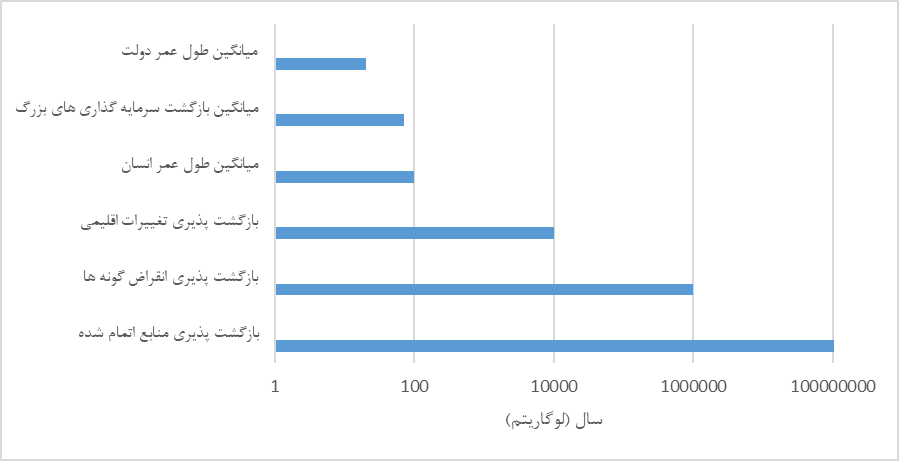
\includegraphics[width=0.9\linewidth]{screenshot001}
	\caption{مقیاس ها برای طبیعت و انسان}
	\label{fig:screenshot001}
\end{figure}
این نمودار بیانگر گستردگی و دامنه آثاری است که نسل امروزی با فعالیت‌های خود بر کره زمین، بر آینده این زیست بوم مشترک بین موجودات زنده می‌گذارد. 

در این گفتار سعی گردیده با توجه به گزارش‌های هیات بین‌الدولی تغییرات‌اقلیمی 
طی سه بند ابتدا به تعریف این پدیده بپردازیم و سپس آثار تغییرات‌اقلیمی را ابتدا بر نظام اقلیم(آثار اولیه) و سپس بر جوامع انسانی(آثار ثانویه) شرح دهیم.









	\subsection*{بند اول: تعریف}\addcontentsline{toc}{subsection}{بند اول: تعریف}
	در این گفتار ابتدا وجوه تماییز تغییرات‌اقلیمی و تغییرات آب‌و‌هوایی مورد بررسی قرار گرفته و سپس با شرح علل این تغییرات، این مفهوم را تعریف نموده‌ایم.


		\subsubsection*{ اول: تغییرات‌اقلیمی یا آب‌و‌هوایی}\addcontentsline{toc}{subsubsection}{ اول: تغییرات‌اقلیمی یا آب‌و‌هوایی}
		میان این دو، اگر چه در ادبیات حقوقی گاها به جای یکدیگر بکار برده می‌شوند، تفاوت وجود دارد. تغییرات آب‌و‌هوایی\LTRfootnote{Weather change.} به رشته‌ای از تغییرات گفته می‌شود که بر سردی و گرمی هوا، کمی و زیادی برف و باران، شدت و ضعف طوفان‌ها و گرد‌باد‌ها در طول چند روز و چند هفته تاثیر می‌گذارد. دانش هواشناسی به پیش بینی آنچه در کوتاه مدت در جو زمین اتفاق می‌افتد، می‌پردازد. 
		
		وقتی از تغییرات‌اقلیمی\LTRfootnote{Climate Change.} صحبت می‌کنیم، تغییراتی مد نظرمان می‌باشد که در بازه طولانی الگو و میانگین آب و هوای روزانه را متاثر می‌کند. امروزه، کودکان مدام روایت‌هایی از پدران و مادران‌شان می‌شنوند که گویای بارش چند متری برف و گاها تونل زدن زیر مسیر‌های برفی و تعطیلی چند روزه مدارسشان در گذشته می‌باشد. در اکثر مناطق کشور کودکان دیگر امکان دریافت چنین تجربه‌هایی را ندارند. این تغییر الگوی بارش برف به خوبی گویای اقلیم تغییر یافته از زمانی که والدین‌شان جوان بودند، می‌باشد.\LTRfootnote{Weather or Climate change, 09-2017, Retrieved from: www.climate.nasa.gov.} 
		
		اگر تابستان‌ها گرمتر از گذشته به نظر می‌رسند و یا وقتی می‌شنویم که مردم در نقاط مختلف جهان ادعا می‌کنند که بهار زودتر از سی سال گذشته رخ می‌دهد. در می‌یابیم که در الگو و نظم اقلیم جهانی تغییراتی بوجود آمده است.
		
		آب و هوا در واقع، شیوه رفتار اتمسفر است با در نظر گرفتن تاثیری که بر زندگی و فعالیت‌های انسان دارد. تفاوت آب و هوا با اقلیم در این است که آب و هوا شامل تغییرات کوتاه ( چند دقیقه تا چند ماه) در اتمسفر است. اقلیم اما میانگین وضعیت آب و هواست در بازه طولانی زمان و فضا. اقلیم آن چیزی است که ما انتظارش را داریم مانند یک تابستان گرم، اما آب و هوا وضعیتی می‌باشد که دریافت می‌کنیم.\LTRfootnote{Roda, Verheyen, \textbf{Climate Change Damage and International Law Prevention Duties and State Responsibility}, Martinus Nijhoff Publishers, 2005, p. 12-13}  















		\subsubsection*{ دوم: تغییرات‌اقلیمی و علل آن}\addcontentsline{toc}{subsubsection}{ دوم: تغییرات‌اقلیمی و علل آن}
		دمای کره زمین وابسته به میزان ورود و خروج انرژی به نظام زمین است. هنگامی که انرژی خورشید جذب زمین می‌شود، زمین گرم گردیده و هنگامی که این انرژی توسط زمین به فضا منعکس می‌شود، زمین شروع به سرد شدن می‌کند. عوامل متعدد طبیعی و انسانی در ایجاد تغییر در چرخه توازن انرژی کره زمین ایفای نقش می‌کنند که شامل: 1- اختلاف میزان انرژی خورشید، 2- تغییرات در میزان انعکاس انرژی وارد شده، از زمین به فضا و 3- تغییرات در اثر‌گلخانه‌ای، که بر میزان گرما کره زمین تاثیر می‌گذارد. این عوامل باعث تغییرات در اقلیم به صورت متعدد می‌شوند.\LTRfootnote{«Causes of Climate Change», 06-2017, Retrieved from: www.archive.epa.gov.}
		اقلیم دارای نظامی پویا و در حال تحول و تغییر بوده، که در تاریخ زمین قابل مشاهده است. این تغییرات که موقت یا با بازه زمانی طولانی و در یک نقطه یا در تمامی سطح کره مسکون رخ می‌دهند، در سه دسته قابل تقسیم بندی می‌باشند. این سه دسته عبارتند از: 1- پروسه‌های طبیعی داخلی 2- تاثیرات انسانی و 3- فشار.
		
		تغییرات ایجاد شده بوسیله فشار در نظام اقلیم، می‌تواند هواویز‌های منتشر شده از سنگ‌های آتشفشانی بوده باشد، یا اینکه بدون فشار خارجی و  به عنوان نمونه در اثر پدیده ال‌نینو باشد. برای مشخص شدن حدود این متن لازم است تمایز قائل شویم میان تغییرات طبیعی اقلیمی، و تغییراتی که در اقلیم بوسیله انسان ایجاد می‌گردد. کنوانسیون چارچوبی تغییرات‌اقلیمی سازمان ملل متحد،\LTRfootnote{United Nations Framework Convention on Climate Change (UNFCCC)} تغییرات‌اقلیمی را به شرح زیر تعریف نموده است: «تغییرات‌اقلیمی به تغییراتی که مستقیما یا با واسطه توسط فعالیت‌های انسان در اقلیم ایجاد گردیده و نسبت اجزای سازنده اتمسفر جهانی را دگرگون می‌نماید گفته می‌شود.»
		
		این تغییرات افزون بر تغییرات‌اقلیمی ایجاد شده بواسطه طبیعت می‌باشد و قابل ارزیابی در بازه زمانی مشخص است. گاهی اوقات به این پدیده تغییرات‌اقلیمی انسان‌آورد گفته می‌شود، تا به خوبی تمایز تغییرات‌اقلیمی طبیعی و انسانی را بیان کند. اشاره به چنین تفاوتی از این باب حائز اهمیت می‌باشد که الزامات حقوقی و مسئولیت را صرفا به انسان می‌توان اختصاص داد. برای این منظور باید تاثیر انسان بر پدیده تغییرات اقلیم را در پس‌زمینه آثار طبیعت بر این پدیده شناسایی نمود.\LTRfootnote{Ibid., p. 13-17.}  
		
		اكسیژن، نیتروژن، و آرگن روی هم رفته 96/99 درصد از جو را تشكیل مى دهند. این گازها در سرمایش و گرمایش زمین نقش زیادى ندارند. 4/0 دهم درصد باقى مانده را، به ترتیب اهمیت، كربن دى اكسید، متان، نیتروزاكسید، ازن، و كلروفلوروكربن‌ها تشكیل مى دهند. این گازها، تابش خورشید را از بالاى جو به پایین راه مى دهند، ولى مانع خارج شدن تابشِ میكرومترىِ زمین به فضا می‌شوند. این گازها، نقشى مانند شیشه در دیوارها و سقف گل خانه دارند و به همین سبب به گازهاى گلخانه اى معروف‌اند. اگر مقدار این گازها در جو بالا رود، زمین گرم می‌شود.\RTLfootnote{ ثبوتی، یوسف، «اقلیم و تغییرات آن در سده‌های بیستم و بیست و یکم»، فصلنامه نشاء علم، سال اول، شماره 2، خرداد 1390، ص. 9-10.}
		
		كربن دى اكسید، بیشتر از سوختن سوخت‌هاى فسیلى و غیرفسیلى، از دم و بازدم موجودهاى زنده، از تبدیل سنگ‌هاى كربن دار به تركیب‌هاى سیلیسى در طبیعت و در صنعت سیمان نشر مى شود. از سوى دیگر، كربن دى اكسید به وسیله روییدنى‌ها، مرجان‌ها و موجودهاى دریایىِ صدف دار جذب مى شود و در آب اقیانوس‌ها به خوبى حل مى شود. متان، بیشتر از تجزیه تركیب‌هاى آلى گیاهى و حیوانى در مرداب‌ها، كف دریاها و جنگل‌ها و نشخوار نشخواركننده‌ها منتشر می‌شود. نیتروزاكسید در طبیعت بوجود مى‌آید و از بین مى‌رود. مصرف روزافزون سوخت‌هاى فسیلى و كودهاى شیمیایى به افزایش آن در جو كمك مى‌كند. ازن در لایه‌هاى بالاى جو در اثر تابش فرابنفش خورشید بوجود مى‌آید و اثر خنك كنندگى دارد. ولى، در لایه‌هاى پایین جو و سطح زمین، ازن در انجام فرآیندهاى صنعتى، مانند جوشكارى و جرقه‌هاى الكتریكى تولید مى‌شود و گرم کننده جو و زمین است. كلروفلوروكربن‌ها به طور طبیعى به وجود نمى‌آیند. انسان ساخت هستند و در افشانه‌ها و ماشین‌هاى سرمازا به‌ كار می‌روند. پیمان نامه‌هاى بین‌المللى،\RTLfootnote{در سال ۱۹۸۵ کنوانسیون وین برای حفاظت از لایه ازن توسط سازمان ملل متحد و دیگر کشورها تدوین شد و سپس در سال ۱۹۸۷ پروتکل مونترال در سازمان ملل متحد توسط ۴۶ کشور پذیرفته شد.} تولید انواع آسیب رسان آنها را محدود كرده است.\LTRfootnote{Intergovernmental Panel on Climate Change (IPCC), 2007, «The Physical Science Basis», Cambridge University Press.}
		
		
		بیش از 20 درصد از کربن دی اکسید اضافه شده در جو به مدت بیش از 1000 سال باقی می‌ماند. انتشار سالانه کربن دی اکسید از سوخت‌های فسیلی و تولید سیمان در سال 2011 به میزان 9.5 گرم بوده است که 54 درصد بالاتر از سطح 1990 می‌باشد. در جهان، انتشار گازهای گلخانهای از سال 1970 به حدود 75 درصد افزایش یافته است.
		















	\subsection*{بند دوم: تاثیرات تغییرات‌اقلیمی  بر نظام اقلیم}\addcontentsline{toc}{subsection}{بند دوم: تاثیرات تغییرات‌اقلیمی  بر نظام اقلیم}
	
	
	
	مشاهدات نظام اقلیم مبتنی بر‌اندازه گیری‌های مستقیم و سنجش از راه دور از ماهواره‌ها و دیگر نظام عامل‌ها است. مشاهدات جهانی در مقیاس وسیع در اواسط قرن نوزدهم برای دما و سایر متغیرها آغاز شد و مجموعه‌های گسترده تر و متنوعی از مشاهدات در دسترس برای دوره 1950 به بعد وجود داشت. تجدید ساختارهای آب‌و‌هوایی که در یک زمان خاص در گذشته زمین‌شناسی شایع است حکایت از برخی از رکورد‌ها دارد که صدها تا میلیون‌ها سال پیش وجود داشته است. با هم، آنها دیدگاه جامع از تغییرات و تغییرات درازمدت در جو، اقیانوس، کریوسفر و سطح زمین را ارائه می‌دهند.\LTRfootnote{Intergovernmental Panel on Climate Change 2013 (IPCC), The Physical Science Basis, Cambridge University Press, p. 4.}
	
	گرم شدن نظام اقلیم که از دهه 1950 شروع شده است در طول دهه‌ها تا هزاران سال پیش بی سابقه بوده است. جو و اقیانوس گرم شده‌اند، میزان برف و یخ کاهش یافته است، سطح دریا و غلظت گازهای گلخانهای افزایش یافته است.
	
	
	
	
	
	\begin{enumerate}
		
		
		
		
		
		
		
		
		\item  جو\\
		هرکدام از آخرین سه دهه در سطح زمین به طور پیوسته گرمتر از سال‌های 1850 بوده است . در نیمکره شمالی، سالهای 2012-1983، احتمالا گرمترین دوره 30 ساله 1400 سال گذشته بود. دمای ترکیبی سطح اقیانوس و  زمین در سطح جهانی و داده‌هایی که به وسیله یک روند خطی محاسبه شده است، در طول دوره زمانی 1880 تا 2012، گرم شدن $ 0.85 $ درجه سانتیگراد را نشان می‌دهد. افزایش کلی دما بین میانگین 1900-1850 و دوره 2012-2003، $ 0.78 $ درجه سانتیگراد است، که مبتنی بر طولانی ترین داده‌های موجود در دسترس است. وقتی محاسبه آمار منطقهای به‌ اندازه  کافی انجام شد، تقریبا تمام سطح زمین گرما را تجربه نموده بودند. تقریبا مطمئن هستیم که گشت کره\LTRfootnote{Troposphere.}  (صفر تا 10 کیلومتری زمین) از اواسط قرن بیستم میلادی گرم گشته است. افزایش روز‌ها و شب‌های گرم و کاهش روز‌ها و شب‌های سرد در سطح جهانی بسیار محتمل است.\LTRfootnote{Ibid, p. 5-7.}
		
		
		
		
		
		
		
		
		
		
		
		
		
		
		
		
		\item	 اقیانوس\\
		تقریبا مطمئن هستیم که بخش بالایی اقیانوس\LTRfootnote{Upper Ocean.} (700-0 متر) از سال 1971 تا 2010 گرم شده است. در مقیاس جهانی، نزدیکترین سطح آب(75 متر)، در سال‌های 1971 تا 2010 با 11/0 درجه سانتیگراد در هر دهه گرم گردیده است. بیش از 60 درصد از انرژی خالص در نظام اقلیمی در اقیانوس بالا در طی نمونه دوره نسبتا خوب 40 ساله از سال 1971 تا 2010 ذخیره گردیده و حدود 30 درصد در بخش زیرین اقیانوس (زیر 700 متر) ذخیره می‌شود. افزاش دما در بخش بالایی اقیانوس در این دوره پیش بینی می‌شود. احتمال زیادی وجود دارد که از سال 1950 در مناطقی با تبخیر بالا شوری غالب باشد، و در مناطقی با بارش زیاد شوری کمتر گردد. این آمار منطقهای به صورت غیر مستقیم بیانگر این نکته می‌باشد که روند تبخیر و بارندگی در اقیانوس‌ها تغییر نموده است.\LTRfootnote{Ibid, P. 8.}
		
		
		
		
		
		
		
		
		
		
		
		
		
		
		
		
		
		
		
		\item  سرماکره\RTLfootnote{سرماکره (Cryosphere)، برف و یخ یخپال‌های کوهستانی و قطب ها و زمین‌های یخ زده را شامل می‌شود.}\\
		در طول دو دهه گذشته، ورقه‌های یخ گرینلند و قطب جنوب، بشدت کاهش یافته‌اند. یخچال‌ها تقریبا در سراسر جهان در حال کاهش بوده‌اند. و پوشش برف بهار و یخ دریای قطب شمال در نیمکره شمالی همچنان در حال کاهش می‌باشد. میانگین افت یخ در یخچال‌های طبیعی در سراسر جهان، به استثنای یخچال‌های طبیعی در حاشیه یخچال‌های یخ، احتمالا 226 میلیون تن\RTLfootnote{افت 100 میلیون تن یخ در سال، معادل 28/0 میلیمتر افزایش سطح آب دریا می‌باشد.}  در سال‌های 1971 تا 2009 می‌باشد. 
		
		صفحات یخ گرینلند و قطب جنوب، بزرگترین اجرام یخ در جهان هستند و در نظام اقلیمی جهانی، نقش مهمی ایفا می‌کنند. هر دو ورقه یخ از سال 1992 مقدار زیادی از یخ را از دست داده‌اند. افت یخ تجمعی از گرینلند از سال 1992 تا 2015 به 3600 گیگاتن رسید و موجب افزایش سطح جهانی آب دریا در حدود 10 میلیمتر شد. شکل مربوطه برای قطب جنوب 1500 گیگاتن است که مربوط به حدود 5 میلیمتر افزایش سطح جهانی آب دریا از سال 1992 است. پیش بینی‌های مدل کاهش بیشتر یخ قطبی در آینده را نشان می‌دهد، اما این موضوع همراه با یک عدم اطمینان بزرگ است. برابر تخمین‌ها ذوب ورقه‌های یخ قطبی تا 50 سانتی متر افزایش سطح دریا در طول قرن 21 را در پیش خواهد داشت. پیش بینی‌های بسیار طولانی مدت (تا سال 3000) نشان دهنده افزایش چند متری سطح دریا، با ذوب شدن ورقه‌های یخ است.\LTRfootnote{Greenland and Antarctic ice sheets, 20 Dec 2016, Key messages, Retrieved from: www.eea.europa.eu, 05/09/18.}
		
		میزان پوشش برف نیمکره شمالی از اواسط قرن بیستم کاهش یافته است. میزان بارش برف نیمکره شمالی در ماه مارس و آوریل به میزان 1.6 درصد و در ماه ژوئن 11.7 درصد در هر دهه در طول دوره 1967 تا 2012 کاهش یافت. در طول این دوره، میزان پوشش برف در نیمکره شمالی در هر ماه افزایش قابل ملاحظهای نشان نداد. با اطمینان بالایی میتوان ادعا نمود که از اوایل دهه 1980 دمای هوا در سراسر جهان افزایش یافته است. گرم شدن مشاهده شده در مناطق آلاسکا شمالی به 3 درجه سانتیگراد (اوایل 1980 تا اواسط سال 2000) و در قسمت شمالی اروپایی روسیه تا 2 درجه سانتیگراد (1971 تا 2010) بود. در منطقه دوم، در طول دوره 1975 تا 2005، کاهش قابل توجهی در ضخامت مرجان و رسوبات مشاهده شده است.\LTRfootnote{Intergovernmental Panel on Climate Change 2013 (IPCC), Op.cit., P. 9.}
		
		
		
		
		
		
		
		\item  سطح دریا\LTRfootnote{Sea Level.}\\
		هیات بین‌المللی تغییرات‌اقلیمی با سطح بالایی از اطمینان، افزایش سطح آب دریا از اواسط قرن 19 نسبت به سطح آن در دو هزاره قبلی را تایید می‌کند. سطح آب دریا از 1901 تا 2010، چیزی حدود 19/0 میلیمتر افزایش یافته است. اطلاعاتی که از سطح دریا با گذر از قرن 19 و در ابتدای قرن 20 وجود دارد بیانگر این امر است که سطح آب دریا از کم به زیاد طی دو هزاره گذشته افزایش یافته است. 
		
		از اوایل دهه 1970، افت انبوه جرم یخچال و انبساط دمایی اقیانوس، که ناشی از گرمایش جهانی می‌باشد، حدود 75 درصد از افزایش سطح جهانی دریا را توضیح می‌دهد. در طول سالهای 1993 تا 2010، افزایش جهانی سطح دریا در مقایسه با مجموع سهم مشاهده شده از انبساط دمایی اقیانوس به علت گرم شدن1/1 میلیمتر در سال، از تغییرات یخچالهای طبیعی76/0 میلیمتر در سال، صفحات یخ گرینلند 33/0 میلیمتر در سال، ورق یخ قطب جنوب27/0 میلیمتر در سال و ذخیره آب زمین38/0 میلیمتر در سال بوده است، که مجموع این سهم‌ها عبارتند از 8/2 میلیمتر در سال. با اطمینان بالایی دریافته‌ایم که حداکثر میانگین جهانی سطح دریا در طول آخرین دوره بین‌یخبندانی، (116000 تا 129000 سال پیش) برای چندین هزار سال، حداقل و حداکثر به ترتیب 5 و 10 متر بالاتر از حال حاضر بوده است.\LTRfootnote{Ibid, P. 11.}
		همچنین علت دیگر افزایش سطح آبها این است که با گرم شدن اقیانوس ها، آب منبسط شده و سطح گسترده تری را پوشش می‌دهد.\LTRfootnote{Islands disappear under rising seas, 4 november 2018, Retrieved from: news.bbc.co.uk, (14 june 1999).}
		
		سطح آب های دریا انتظار می‌رود که در سال 2100 با درجه گرمای 5/1 سانتی گراد کره زمین چیزی حدود 1/0 متر کاهش یابد. سطح آب ها حتی بعد از سال 2100 به افزایش خود ادامه خواهد داد. اندازه و نرخ رشد سطح آبها به میزان کاهش یا افزایش انتشار گاز های گلخانهای توسط نسل امروز و نسل های آینده وابسته می‌باشد. بدیهی است نرخ رشد پایین تر سطح آبها فرصت های بسیاری را برای انطباق با شرایط جدید به انسان می‌دهد.\LTRfootnote{Intergovernmental Panel on Climate Change(IPCC), «Summary for Policymakers», 2018, P. 9.}
		
		
		
		
		
		
		
		
		
		
		\item کربن و دیگر چرخه های زیست گیاه شناسی\LTRfootnote{Carbon and Other Biogeochemical Cycles.}
		
		غلظت اتمسفر از دی اکسید کربن، متان و اکسید نیتروژن به سطح بی سابقه ای، در حداقل 800000 سال گذشته افزایش یافته است. غلظت دی اکسید کربن از زمان‌های قبل از صنعتی‌شدن 40درصد  افزایش یافته است، که این میزان در درجه اول ناشی از انتشار سوخت‌های فسیلی و درجه دوم از تولید گازهای گلخانهای ناشی از تغییر کاربری اراضی خالص می‌باشد. اقیانوس حدود 30‌درصد از دی اکسید کربن تولید شده انسانی را جذب کرده است، رخدادی که منجر به اسیدی شدن اقیانوس می‌شود.
		
		غلظت گاز‌های گلخانهای همچون کربن‌دی‌اکسید، متان و اکسید‌نیتروژن، از زمان 1750 به علت فعالیت‌های انسانی افزایش یافته است. در سال 2011، غلظت این گاز‌ها، به ترتیب 391 بخش در میلیون، 1803 و 324 بخش در میلیارد بود، که حدودا 40، 150 و 20 درصد بیشتر از مقادیر دوره پیشاصنعتی می‌باشد. غلظت کربن‌دی‌اکسید، متان و اکسید‌نیتروژن، در حال حاضر به طور قابل ملاحظهای بیش از بالاترین غلظت ثبت شده در هسته یخ طی 800000 سال گذشته است.متوسط افزایش غلظت این گاز‌ها در جو در طی قرن گذشته، در 22000 سال گذشته بی‌سابقه بوده است.
		
		اسیدی شدن اقیانوسها با کاهش 
		\LTRfootnote{potential of hydrogen PH \persian(یک کمیت لگاریتمی است که میزان اسیدی یا بازی بودن مواد را مشخص می‌کند.)}
		PH مشخص می‌گردد. pH آبهای سطحی اقیانوس از زمان آغاز عصر صنعتی 1/0 درصد کاهش یافته است، که مربوط به افزایش 26 درصدی غلظت یون هیدروژن است.\LTRfootnote{Ibid, P. 12.}
	\end{enumerate}
	
	
	
	\subsection*{بند سوم: تاثیرات تغییرات‌اقلیمی بر جوامع انسانی}\addcontentsline{toc}{subsection}{بند سوم: تاثیرات تغییرات‌اقلیمی بر جوامع انسانی}
	
		
		
\begin{enumerate}
	
			\item	تاثیر تغییرات‌اقلیمی بر نیاز‌های اولیه\\
نیاز‌های اولیه مورد اشاره شامل کشاورزی، تامین و کیفیت آب، سلامتی و مسکن می‌باشد، که مورد بررسی واقع می‌شود. 
				\begin{itemize}
					\item کشاورزی و خوراک\\
تغییرات در اقلیم تاثیر بسزائی در تولید مواد غذایی در سراسر کره زمین داشته است. استرس گرما، خشکسالی و سیلاب‌ها منجر به کاهش محصولات زراعی و تولیدات دامی می‌شود. مناطقی از کره که هم اکنون متاثر از خشکسالی می‌باشند مانند استرالیا و بخشی از آفریقا که در جنوب صحرای کبیر قرار دارد، مشکل کمبود آب در دسترس برای آبیاری را تجربه خواهند نمود.

در عرض جغرافیایی متوسط تا بالا پیش بینی می‌شود که رویش محصولات زراعی قَله با توجه به میزان گرمای منطقه و نوع محصول به آرامی افزایش یابد. در عرض‌های جغرافیایی کمتر، محصولات کشاورزی قَله کاهش خواهد یافت. بیشترین کاهش در محصولات قَله در مناطقی با آب و هوای خشک و استوایی رخ خواهد داد. به عنوان نمونه تا سال 2050 پیش بینی می‌شود که در برخی کشور‌های آفریقایی کاشت و برداشت محصول گندم بیش از 35 درصد، کاهش یابد. \LTRfootnote{Intergovernmental Panel on Climate Change 2014 (IPCC), «Impacts, Adaptation, and Vulnerability Part B: Regional Aspects», Cambridge University Press, United States of America, P. 1218.}

تغییرات‌اقلیمی بر صنعت شیلات در عمده مناطق کره زمین تاثیر گذاشته است. افزایش دمای اقیانوس‌ها باعث شده بعضی گونه‌های دریایی به آب‌های خنک تر تغییر مکان دهند. صنعت شیلات به جهت تامین خوراک و اینکه اقتصاد بسیاری کشور‌ها به آن وابسته می‌باشد، دارای اهمیت است. به عنوان نمونه، خوراک بیش از 40 میلیون انسان وابسته به نوعی ماهی می‌باشد که از دلتای مکونگ\RTLfootnote{ین رود بزرگترین رود آب شیرین برای ماهی گیری در جهان می‌باشد که از تبت سرچشمه گرفته و از چین و هندوچین می‌گذرد و به دریای جنوب چین می‌ریزد} در آسیا، تامین می‌گردد. پیش بینی می‌شود، کاهش جریان آب و افزایش سطح آب دریاها، برکیفیت آب و گونه‌های ماهی در مناطقی مانند نمونه بالا تاثیر منفی خواهد گذاشت، و این عامل بر تامین مواد غذایی جوامعی که به این گونه منابع وابسته می‌باشند، تاثیر خواهد داشت.\LTRfootnote{ Intergovernmental Panel on Climate Change (IPCC) 2014, Op.cit., P. 1355.}

				تغییرات‌اقلیمی امنیت غذایی را در ابعاد جهانی منطقهای و محلی بوسیله اختلال در دسترسی به خوراک، کاهش دستیابی به منابع غذایی و سخت کردن بهره‌برداری تحت تاثیر قرار می‌دهد. ریسک اقلیم در امنیت غذایی برای جمعیت فقیر و مناطق گرمسیری بسیار زیاد می‌باشد.
				\LTRfootnote{International Climate Impact, 06-2017,  Retrieved from: 19january2017snapshot.epa.gov} \\
					\item تامین و کیفیت آب\\
مناطق خشک و نسبتا کم آب مانند منطقه مدیترانه، جنوب آفریقا، و شمال برزیل مستعد تاثیرات تغییرات‌اقلیمی بر تامین آب می‌باشند. در قرن آینده این مناطق، مخصوصا بخش‌هایی که به علت خشکسالی، فشار جمعیت، و بهره‌برداری بی‌رویه منابع آبی، زنگ خطر کم آبی کاهش منابع آبی را تجربه خواهند کرد.

در اثر تغییرات‌اقلیمی، آب در مناطق بسیاری، در حال تبدیل شدن به یک منبع کمیاب است، در حالی که در برخی دیگر مناطق، آب کافی وجود خواهد داشت. دسترسی به آب به میزان بسیاری منوط به میزان بارش نزولات آسمانی و روان آب‌ها می‌باشد. با افزایش 2.7 فارنهایت در دمای جهان میانگین بارش سالانه پیش بینی می‌شود بین 10-50 درصد در عرض جغرافیایی بالا و در برخی مناطق گرمسیری افزایش یابد و در همین حین در مناطق خشک و عرض‌های جغرافیایی متوسط و نیمه حاره همین حدود کاهش یابد.\LTRfootnote{Intergovernmental Panel on Climate Change (IPCC) 2013, Op.cit., P. 91.} با افزایش دما بارش برف در بسیاری مناطق کاهش می‌یابد. یخچال‌های قطب با سرعت بی سابقهای آب می‌شوند و دسترسی به آب را در مناطقی که وابسته به آب شیرین یخچال‌ها در بهار و تابستان هستند محدود می‌سازد. خشکسالی مدام گسترش می‌یابد. افزایش بارش، سطح منابع آب آشامیدنی را افزایش نمی‌دهد بلکه باعث افزایش سیل‌ها می‌شود.

کیفیت آب برای بوم‌سازگان، بهداشت و سلامت بشر، کشاورزی و دیگر اهداف حائز اهمیت است. افزایش دما، تغییر در بارش، افزایش سطح آب و حوادث طبیعی از جمله عوامل تاثیر گذار بر کیفیت آب می‌باشند. طوفان‌های بارانی بسیار بزرگ باعث ورود منابع آلوده کننده به رودخانه‌ها شده و آب زیادی ممکن است نظام فاضلاب و ضربه‌گیر‌های طبیعی را درهم بشکند. افزایش آلودگی مانند افزایش دمای آب می‌تواند عامل افزایش انفجاری رشد جلبک و خزه و افزایش بالقوه باکتری در مجموعه آب شود. در مناطق ساحلی و جزایر کوچک، آب شور ناشی از افزایش سطح آب دریا و موج‌های طوفان امکانات آبی را تهدید می‌کند. این آثار جوامع را ملزم می‌کند تا بدنبال منابع آبی مطمئن برای استفاده بشر باشد.\LTRfootnote{Intergovernmental Panel on Climate Change (IPCC) 2014, Op.cit., PP. 229-269.}
					\item سلامت بشر\\
ریسک بیماری‌ های ناشی از تغییرات‌ اقلیمی در کشور‌هایی که امکانات مناسبی جهت مقابله با بیماری را ندارند بسیار بیشتر می‌باشد. نمونه‌های بسیاری از بیماری‌های مرتبط با تغییرات‌اقلیمی وجود دارد. افزایش دمای کره با استرس گرما به صورت جدی لینک شده است. بدتر شدن کیفیت هوا که معمولا همراه با موج گرما و حریق‌های گسترده رخ می‌دهد منجر به مشکلات تنفسی و تشدید آن و بیماری‌های قلبی می‌شود.\LTRfootnote{Ibid, P. 1057.} اثر تغییرات‌اقلیمی بر کشاورزی و نظام غذایی می‌تواند باعث افزایش نرخ سوتغذیه و بیماری‌های مرتبط با غذای کم کیفیت شود. 

تغییرات‌اقلیمی می‌تواند بر بیماری‌های واگیردار موثر باشد. گسترش بیماری همه‌گیر مننژیت عموما با تغییرات‌اقلیمی مخصوصا خشکسالی لینک شده است. مناطقی در زیر صحرای آفریقا و آفریقای غربی به گسترش مننژیت حساس بوده و به صورت خاص در ریسک می‌باشد اگر خشکسالی گسترش یافته و شدید شود. احتمال گسترش بیماری‌های قابل حمل به وسیله پشه مانند مالاریا، تب استخوان شکن و ویروس غرب نیل  در مناطقی که پیش بینی می‌شود بارش و سیل بیشتری را دریافت می‌کنند وجود دارد. افزایش باران و دما منجر به گسترش بیماری تب استخوان شکن می‌باشد.\LTRfootnote{Ibid, P. 722.} 

تغییر در الگوی بارش و حوادث حاد اقلیمی منجر به کاهش آثار سلامت می‌شود به خصوص هنگامی که قدرت، آب یا نظام حمل و نقل مختل گردد. بیماری اسهال که ناشی از آب آلوده و منابع غذایی می‌باشد به یک نگرانی بزرگ به خصوص برای کودکان تبدیل می‌گردد. اثر تغییرات‌اقلیمی بر سلامت روانی و رفاه، بخش جدایی ناپذیر از مجموعه اثار مرتبط با تغییرات‌اقلیمی بر سلامت بشر می‌باشد. آثار تغییرات‌اقلیمی بر سلامت روانی طیفی از استرس ‌اندک و نشانه‌های اضطرار تا اختلالات بالینی مثل اضطراب، افسردگی، اختلال فشار روانی و افکار خودکشی را شامل می‌شود.\LTRfootnote{Ibid, P. 732.} 

گروه‌های خاصی از مردم در کشور‌های کم درآمد به صورت خاص در معرض آثار معکوس تغییرات‌اقلیمی در سلامت هستند. این گروهای در ریسک شامل مردم فقیری که در شهر زندگی می‌‌کنند، گروه بزرگسالان، کودکان، جوامع سنتی، کشاورزان و جمعیت ساحلی می‌باشند. بسیاری از مناطق مانند اروپا، آسیای جنوبی، استرالیا و شمال آمریکا اثرات بهداشتی مرتبط با گرما را تجربه کرده‌اند. جمعیت روستایی، بزرگسالان، کارگران بیرون خانه و آنهایی که دسترسی به تهویه مطبوع ندارند، بیشتر از دیگران مستعد بیماری و مرگ و میر مرتبط با گرما می‌‌باشند.
					\item مسکن\\
تغییرات‌اقلیمی بر مهاجرت افراد در داخل و بین کشور‌های جهان، تاثیر می‌گذارد. عوامل بسیار زیادی به مهاجرت افراد به مناطق دیگر اثر می‌گذارد. این عوامل می‌تواند شامل اختلافات بر سر منابع، افت خدمات بوم‌سازگان، کمبود زمین کشاورزی بادوام یا آب تازه، و رویداد‌های شدید مانند سیل، خشکسالی و طوفان باشد.\LTRfootnote{Ibid, P. 1353.} 

رویداد‌های شدید، بسیاری از مردم را مخصوصا در مکان‌هایی که مردم توانایی یا منابع برای پاسخ‌گویی و بازسازی پس از فاجعه را ندارند، بی خانمان می‌کند. مدل‌های مختلفی از این قبیل رویداد‌ها، که اختلافات موجود را تشدید می‌کند، به صورت مکرر و شدید در حال رخ دادن است. این خود موجب افزایش میزان مهاجرت‌ها، حین و پس از این رخداد‌ها می‌شود. 

شهرک‌های ساحلی و نواحلی کم ارتفاع به ویژه در برابر تاثیرات تغییرات‌اقلیمی مانند افزایش سطح آب، فرسایش، و طوفان‌های شدید، آسیب پذیر می‌باشند. افزایش دمای اقیانوس و اسیدی شدن آن، همچنین عامل تهدید بوم‌سازگان ساحلی می‌باشد. با نابود شدن زیستگاه‌های ساحلی (مانند جزایر سنگی، تالاب‌ها، دلتا‌ها و مصب‌ها) سکونت‌گاه‌های ساحلی بیشتر در معرض سیل ناشی از طوفان‌های شدید و فرسایش قرار می‌گیرند. هم کشور‌های توسعه یافته و هم در حال توسعه در معرض اثرات افزایش سطح آب می‌باشند.\LTRfootnote{Ibid, P. 381.} 
				\end{itemize}
			\item 	جمعیت آسیب‌پذیر	\\
گروه‌های بومی در مناطق مختلف مانند آمریکا، آمریکای جنوبی و لاتین، اروپا و آفریقا، در حال تجربه تهدیدات مربوط به زندگی سنتی هستند. زندگی بومیانی که در جزایر کم سطح سکنی گزیده‌اند توسط افزایش سطح آب و رویداد‌های شدید تهدید می‌شود. افزایش دما، و کاهش برف، یخ و لایه همیشه یخ بسته زمین گروه‌هایی را که در کوهستان و مناطق قطبی زندگی می‌کنند تهدید می‌کند. تغییرات‌اقلیمی در این مناطق بر شکار، صید، حمل و نقل و دیگر فعالیت‌ها تاثیر می‌گذارد.

تقریبا 4/1 میلیارد انسان، که شامل 5/1 جمعیت کره زمین می‌شود زیر معیار‌های بانک جهانی در مورد فقر و در فقر شدید زندگی می‌کنند. گروه‌های کم درآمد بسیاری وابسته به خدمات و منابع عمومی مانند آب، انرژی و حمل و نقل هستند. حوادث شدید این منابع و خدمات را مختل می‌کند. بسیاری از مردم در کشور‌های کم درآمد امکان دستیابی به مکانیزم‌های انطباق پذیری مانند تهویه مطبوع، گرما یا بیمه حوادث را ندارند. این کمبود ظریفت انطباق پذیری، جمعیت ضعیف زمین را در برابر رویداد‌های شدید اقلیمی آسیب پذیر نموده و با منجر شدن به فقر بیشتر و تثبیت آن، وضعیت این گروه‌ها را تشدید می‌کند. 

بزرگسالان و کودکان نسبت به آثار تغییرات‌اقلیمی همچنین گروه حساس می‌باشند. نظام تنفسی،‌ ایمنی و عصبی در حال توسعه کودکان آنها را نسبت به برخی آثار تغییرات‌اقلیمی همچون حوادث متعاقب و شدید، افزایش گرما و آلودگی شدید هوا بیشتر حساس می‌کند. جمعیت بزرگسال همچنین با توجه به نحیف بودن و تغییر پذیری ‌اندک، در ریسک هستند. گرمای شدید و طوفان می‌تواند به صورت نامتناسب بر گروه بزرگسالان تاثیر بگذارد.\LTRfootnote{Ibid, P. 717-718.} 

تاثیر تغییرات‌اقلیمی با توجه به جنسیت می‌تواند متفاوت باشد. زنان نرخ مرگ و میر بیشتری در اثر طوفان‌ها و رویداد‌های شدید  به نسبت مردان دارند، اگرچه تنوع منطقهای در آمار وجود دارد. در برخی نقاط مردان در سن کاری که خارج از خانه مشغول می‌باشند بیشتر در برابر مرگ و میر ناشی از گرما آسیب پذیر هستند. زنان در کشور‌های در حال توسعه در برابر حوادث شدید با توجه به تفاوت‌های جسمی و میزان فقر و بارداری یا نرسیدن خوراک کافی به بدن گروه آسیب پذیر محسوب می‌شوند.\LTRfootnote{Ibid, P. 635.}
			
			
			
			
			
			
			
			
			
			
			\item 	امنیت ملی	\\
امنیت انسان بستگی به وجود یک نظام دارد که در آن هر فرد عقلانی برابر محاسباتش به این نتیجه برسد که همکاری با نظام بیشتر از شورش، جنگ داخلی، تروریسم، جرم و غیره سود آور است. افراد عقلانی اگر رفاه و امنیت فردی و رونق و امنیت آینده خود را در همکاری با نظام تضمین شده بیابند، به این فعالیت ها اقدام نخواهند کرد. بنابراین، یک نظام امن باید بتواند استاندارد قابل قبول زندگی و وعده یک آینده ی پایدار برای هر فرد را تضمین کند.\LTRfootnote{Gough, Mark, «Human Security: The Individual in the Security Question - The Case of Bosnia», Contemporary Security Policy, V. 23, 2002, PP. 154-155.}

با توجه به تفاوت در تقسیم منابع در سطح کره زمین، تغییرات‌اقلیمی به شیوه های متفاوتی بر امنیت انسانی تاثیر خواهد گذاشت. به عنوان نمونه: خلاف کشورهای صنعتی، که کشاورزی نیازمند یک یا دو درصد از نیروی کار است در کشور‌های شرقی 85 درصد از جمعیت به عنوان اصلی‌ترین منبع درآمد خود به کشاورزی وابسته می‌باشند. اکثر این جمعیت به کشاورزی مشغول هستند به طوری که 46 درصد از مردم روستایی زیر خط فقر و با 55/0 دلار در روز زندگی می‌کنند.\LTRfootnote{Jon Barnett, W. Neil Adger, «Climate change human security and violent conflict», Political Geography, V 26, 2007, P. 641.} 

انتظار می‌رود با افزایش آثار تغییرات‌اقلیمی نگرانی‌ها در خصوص امنیت ملی و آمار درگیری‌های بین‌المللی افزایش یابد. تغییرات‌اقلیمی عامل ناپایداری در کشور‌ها، صدمه در دسترسی به آب و غذا، آسیب دیدن زیرساخت‌ها، شیوع بیماری‌ها، آواره شدن و بی خانمانی گروه بسیاری از مردم می‌باشد.\LTRfootnote{Intergovernmental Panel on Climate Change 2014 (IPCC), Op.cit., P. 733.} 

بسیاری از نگرانی‌ها حول محور منابع طبیعی مانند آب می‌چرخد. در بسیاری از مناطق زمین دسترسی به آب تبدیل به یک معضل محلی و منطقه‌ای شده است. دسترسی به منابع مطمئن آب در این مناطق بسیار با ارزش می‌باشد. تغییرات در میزان و زمان بارش امکان تبدیل شدن محدودیت‌های‌ اندک را به اختلافات آینده ایجاد می‌کند.\LTRfootnote{Ibid, p. 253.}
شواهد نشان می‌دهد بیشترین نزاع ممکن است بین جوامع محلی، گروه‌های اجتماعی-اقتصادی و ایالت/استان‌ها رخ دهد، در حالی که تعاملات دوجانبه و چند جانبه شاهد همکاری رسمی در مورد منابع است.

امنیت غذایی مورد تهدید در برخی بخش‌های آسیا و زیر صحرای آفریقا عامل ایجاد اختلافات می‌باشد. رشد بی رویه جمعیت و تغییرات در میزان بارش و دما در میان دیگر عوامل بر تولید محصولات در حال تاثیر گذاری می‌باشد. نتیجه کمبود مواد غذایی ریسک بحران‌های بشردوستانه و مهاجرت جمعیتی را در مرز‌های ملی افزایش داده و نهایتا یکپارچگی سیاسی کشور‌ها را ناپایدار می‌نماید.

اگر گرم شدن کره زمین بیش از یک آستانه خاص ادامه یابد، که باعث از دست دادن تقریبا کامل یخچال یخ گرینلند در طی یک هزاره یا بیشتر شود، سطح جهانی دریا به صورت متوسط حدود 7 متر افزایش خواهد یافت. آینده تغییرات سطح دریا در حوزه منطقهای متفاوت خواهد بود، اما پیش بینی می‌شود در حدود 70 درصد از خطوط ساحلی، 20 درصد از میانگین جهانی تغییر سطح دریا را تجربه کنند.\LTRfootnote{Ibid, P. 188-189.} از دست دادن مداوم پوشش یخ در قطب اقیانوس اطلس، همراه با پیامد‌های امنیت ملی می‌باشد. اقیانوس اطلس دارای تاریخچهای طولانی از فعالیت نسبتا کم کشتی رانی اگرچه در حال رشد دارد که شامل مسیر‌های حمل و نقل دریایی قطب شمال می‌شود. 

کاهش پوشش یخ دریا به رشد فعالیت‌های دریانوردی می‌انجامد. مسیر شمال-غرب بواسطه تغییرات‌اقلیمی بین آسیا و اروپا برای اولین بار در سال 2007 خالی از پوشش برف گردید.\LTRfootnote{Michael Byers, Suzanne Lalonde, «Who owns the Northwest Passage?», Journal of Transnational Law, v. 42, 2009, P. 1138.}اگر چه شمار زیادی از عوامل بین‌المللی دیگر بر پتانسیل رشد دریانوردی تاثیر می‌گذارد. در مورد اقیانوس قطب شمال، افزایش دریانوردی به معنای اهمیت دوچندان مباحثی همچون حاکمیت (اولویت در کنترل یک منطقه)، امنیت (مسئولیت نظارت بر مسیر‌ها)، حفاظت  محیط‌زیست دریایی (کنترل آلودگی هوا و آبراه کشتی، سرو صدا، صدمه کشتی به وال‌ها) و ایمنی (مسئولیت نجات و پاسخ) می‌باشد.\LTRfootnote{Arctic Council, Arctic Marine Shipping Assessment Report, 2009, Retrieved from: www.pmel.noaa.gov, 9/9/2018, P. 5.} 

همچنین پس از بررسی دانشمندان رابطه میان تاثیر تغییرات‌اقلیمی و ایجاد زلزله بررسی شد. در این بررسی دکتر برندس\LTRfootnote{Brandes.} به همراه تیم خود، بررسی نمودند که آیا آب شدن یخچال های قطب بر تغییر شکل یک منطقه از دانمارک تاثیر گذارده یا نه. آنها دریافتند که در دور پلیستوسن که بین دو نیم میلیون  تا 12 هزار سال پیش ادامه یافته، حرکت و افتادن یخچال ها عامل تحرک و ایجاد زلزله و تغییر فضای دانمارک  بوده است. این تحقیقات اثبات می‌کند که با توجه به فرایند تغییرات‌اقلیمی و سرعت گرم شدن زمین، توجه به  قطب شمال و جنوب و تاثیر افتادن سازه ها و ساختار های یخی آن بر امنیت مناطق و جمعیت انسانی دارای اهمیت زیادی می‌باشد.\LTRfootnote{ Brandes, Christian,  «Can Climate Change Cause Earthquakes?», Aug 15, 2018, Retrieved from: www.scientia.global.} 
	در اقیانوس آرام، یک سوم سواحل از 200 جزیره مالدیوی که مسکونی نیز می‌باشند به زیر آب رفته‌اند.
	\LTRfootnote{Islands disappear under rising seas, Op.cit..}
	
	
\end{enumerate}


\section*{گفتار سوم: حق بر آینده سبز}
\addcontentsline{toc}{section}{گفتار سوم: حق بر آینده سبز}
در این گفتار، مفاهیم آینده سبز، کودک و نسل‌های آینده در سه بند از نظر لغوی تعریف گردیده و حدود آنها مشخص می‌شود. 

	\subsection*{بند اول: آینده سبز}\addcontentsline{toc}{subsection}{بند اول: آینده سبز}

%در این بند، آنچه مورد توجه می‌باشد مفهوم آینده سبز\RTLfootnote{عبارت حق بر آینده سبز از کتاب زیر گرفته شده است.\latin{Hiskes, Richard P., \textbf{The Human Rights to a Green Future}, Cambridge University Press, United State, 2008.}} است. از این مفهوم در متون علمی کمتر سخن رفته است. 

حق بر آینده سبز، مفهومی خود ساخته است. نگارنده در این بند در پی آن است که به این پرسش پاسخ دهد که آیا حق بر آینده سبز باید وجود داشته باشد؟ اگر قائل به چنین حقی باشیم باید پرسید چه افرادی از این حق بهره خواهند برد؟ در ادامه تلاش شده که این موضوع تشریح گردد. 

در دو گفتار قبل سعی نمودیم به چالش‌های نو ظهور در حوزه محیط‌زیست بپردازیم. نتیجه این بررسی این شد که در زمانه حاضر عناصری از طبیعت که بین عموم موجودات مشترک است به صورت بلند مدت تخریب شده است. اقلیم در محدوده چند صد سال آینده تحت تاثیر رفتار نسل‌های گذشته و حاضر خواهد بود و در واقع، مبتنی بر آثار و گزارش‌های علمی موجود، نسل‌های آینده چالش‌هایی را تجربه خواهند نمود که مسئول آن نسل حاضر است. 

ولفگانگ فیکِنچِر، در نظریه خود(یافتن و معنا کردن زمان گذشته در آینده) به ایستایی و پویایی حقوق پرداخته و نسیم زمان را در نظریه خود، به پیش جریان داده است. به اعتقاد وی قانون در حکم یا فرمانِ قطعی خود بازنمای حقوقِ بی حرکت است؛ تصویری است از یک لحظه منفرد. اما حقوق باید در لحظات همیشه نو، در زمان و در تاریخ تحقق یابد.\footnote{فلسفی، پیشین، صص. 96-98.}

این نظریه، ذهن حقوق‌دان را منعطف می‌کند به شرح و بسط دادن حقوق به شیوه‌ای که حقوق فراتر از احکام یا فرمان‌های کلی مندرج در متن قانون باشد و با این اندیشه که نظام دستوری(نورماتیو) بالاتر از حد توقعات زمان‌های تغییر پذیر قرار بگیرد. وی بیان می‌کند که متصدی حقوقی باید مضمون قاعده کلی و ایستا را در مقابل وجوه واقعی و پویای زندگی خم کند. به این فن و روش تغییر و تبدیل، ایجاد قاعده مرتبط با مورد می‌گویند.\footnote{پیشین.}


در متن حاضر حق بر آینده سبز به مجموعه حقوق و منافعی اشاره دارد که در آینده برای آیندگان قابل حصول می‌باشد.(حقی که مبتنی بر مورد(چالش‌های تغییرات‌اقلیمی در آینده) ایجاد می‌شود.) محوریت و مبنا این حقوق و منافع، باید با توجه به اصول و آرمان‌هایی  همچون بشریت و عدالت ‌باشد.  %انتخاب این مفهوم به جهت پرهیز از ترکیب واژگان حق و نسل‌های آینده (به دلیل عدم استفاده از آن در اسناد حقوقی ) می‌باشد. دلیل عدم اشاره به نسل حاضر دو امر می‌باشد یکی اینکه نسل بالغ حاضر خود در نقش تاثیر گذار و عامل در عرصه زندگی حضور دارد، در حالی که کودکان و نسل‌های آینده به ترتیب اهلیت استیفا و حضور برای ایفای نقش ندارند اما همانطور که خواهیم دید متاثر از تغییرات‌اقلیمی خواهند بود. دومین علتِ عدم اشاعه موضوع به نسل بالغ حاضر، توجه به بازه زمانی تاثیراتی می‌باشد که تغییرات‌اقلیمی در کره زمین ایجاد می‌نماید.\footnote{به شکل شماره 1 رجوع شود.}  بنابراین

بنابراین، به صورت خلاصه باید گفت با توجه به ایجاد چالش‌های بلند‌مدت در آینده توسط تغییرات‌اقلیمی، حق بر آینده سبز که از آرمان بشریت و عدالت ریشه می‌گیرد، بوجود می‌آید. 
مراد از حق بر آینده سبز در این متن مجموعه منافعی می‌باشد که کودکان و نسل‌های آینده در حوزه  محیط‌زیست برای زندگی بدان نیاز خواهند داشت. 





در خصوص ارتباط میان انسان و  محیط‌زیست سه رویکرد مختلف وجود دارد. 1- رویکرد انسان محوری محض و سخت؛ طبق این رویکرد هدف اصلی، دسترسی و بهره‌برداری فوری از منابع طبیعی است. و نگاه انسان به  محیط‌زیست  تنها برای رفع نیاز‌ها و بهره‌برداری اقتصادی صرف از آن می‌باشد. 2- رویکرد  محیط‌زیست محوری؛ خلاف رویکرد انسان محوری محض و سخت، در این رویکرد انسان به عنوان بخشی از  محیط‌زیست به شمار می‌آید که باید همانند سایر اشکال حیات و بدون توجه به بهرهای که برای انسان دارد، مورد پشتیبانی قرار بگیرد. 3- عدالت محیط‌زیستی؛ عدالت محیط‌زیستی بر سه جنبه عدالت میان انسان‌ها در تقسیم بهره‌مندی از  محیط‌زیست، عدالت میان نسل‌های کنونی و آینده و عدالت میان گونه‌ها (انسان و دیگر گونه‌ها) تاکید دارد.\footnote{رمضانی قوام آبادی، محمد حسین، از ریو تا ریو:در تکاپوی توسعه پایدار، مجله تحقیقات حقوقی، شماره 62، تابستان 1392، ص 414.}  
	
	
	\subsection*{بند دوم: کودک}\addcontentsline{toc}{subsection}{بند دوم: کودک}
واژه کودک که برابر آن بچه می‌باشد به فرزند انسان خواه دختر یا پسر اطلاق می‌شود. علت به کار بردن واژه کودک برای فرزند انسان اعلام عدم رشد وی می‌باشد.\footnote{معین، محمد، \textbf{فرهنگ معین}، جلد دوم، چاپ چهارم، انتشارات اَدِنا، تهران، 1381، ص 313.} کودک به جهت عدم رشد شخصیتی در برابر قانون دارای وضعیتی متفاوت از بزرگسالان می‌باشد. به صورتی که از طرفی حقوق متفاوتی به او اختصاص پیدا می‌کند و از طرف دیگر تکالیف و مسئولیت او متناسب وی باید باشد. در این میان لازمه ایجاد نظم در جامعه در نظر گرفتن معیاری برای تمایز کودک از بزرگ سال به جهت تمایز حقوق و تکالیف آنها است.  کودک در علوم مختلف انسانی دارای تعاریف متفاوتی می‌باشد. عدم انطباق تعاریف با یکدیگر و تاثیر آن در عالم حقوق آنجا که از طرفی کودک را مسئول نمی‌دانیم و در صدد حمایت از او هستیم ایجاب می‌نماید تا محدوده کودکی با واقعیات تبیین گردد. 

رشد امری تدریجی می‌باشد و به یک باره حاصل نمی‌آید تا بتوان گفت فرد با رسیدن به سن مشخصی حتما رشد را به همراه داشته باشد و از شمول لفظ «کودک» خارج گردیده است. اما همین واقعیات اجتماعی ایجاب می‌نماید که معیاری را به عنوان اماره‌ای نسبی در جهت تفکیک کودک و بزرگسال قرار دهیم. در تعیین این معیار باید به کلیه جنبه‌های روحی، روانی و جسمی فرد انسان توجه شود و معیاری تعیین شود که با غالب افراد جامعه منطبق باشد.\footnote{ اسدی، لیلا سادات،«بررسی مفهوم کودک با رویکردی به حوزه کیفری»، نشریه فقه و حقوق خانواده(ندای صادق سابق)، سال دوازدهم، بهار وتابستان 86، ص. 38.} 

هر چند در اسناد، اعلامیه‌ها و معاهدات بین‌المللی واژه کودک به کرات مورد استفاده قرار گرفته اما تعریفی که بیانگر اتفاق نظر جهانی باشد وجود ندارد. به موجب ماده یک کنوانسیون حقوق کودک:« کودک یعنی هر انسان زیر 18 سال» با این تعریف هرچند تدوین کنندگان کنوانسیون حقوق کودک معیاری مطمئن برای تشخیص کودک از بزرگسال تعیین نموده‌اند، اما با آوردن قید «مگر اینکه بر طبق قانون مربوط، سن بلوغ کمتر باشد» به دولت‌ها اجازه داده شده تا سن دیگری را برای کودکی مشخص نمایند.\footnote{
	ابراهیمی، زهرا، (1393)، حق سلامت کودک در نظام بین‌المللی حقوق بشر، پایان نامه کارشناسی ارشد حقوق بشر، دانشگاه شهید بهشتی.
}  البته در ماده 2 منشور آفریقایی حقوق و رفاه کودک\LTRfootnote{African Charter on the Rights and Welfare of the Child, } این قید حذف گردیده و در بیان مفهوم کودک آمده که از نظر این منشور کودک هر شخص انسان زیر 18 سال می‌باشد. 

ماده یک میثاق حقوق کودک در اسلام، کودک را چنین تعریف نموده است: «منظور از کودک هر انسانی است که بر اساس قانون قابل اعمال در مورد وی به سن بلوغ نرسیده باشد.» در این میثاق معیار تمایز دوران کودکی و بزرگسالی بلوغ شخص می‌باشد نه رسیدن به سنی معین. از این منظر شخص رشد نایافته برابر کودک بوده و بلوغ مرحلهای از رشد جسمانی و عقلانی در نظر گرفته شده که پس از آن شخص دارای اهلیت استیفا و توانایی انجام امور خود به صورت مستقل می‌گردد. 

با وجود در نظر گرفتن معیار‌های مختلف در اسناد بین‌المللی برای تعیین دوران کودکی، در این پژوهش با عنایت به کنوانسیون حقوق کودک، مقصود از کودک افراد زیر 18 سال سن می‌باشند. با مشخص شدن دوران پایان کودکی، شروع آن نیازمند بررسی می‌باشد. اعلامیه جهانی حقوق بشر در ماده 1 خود تصریح نموده که انسان‌ها از لحظه تولد حقوق و منزلت برابر دارند. سوالی که ذهن را درگیر می‌کند این است که آیا جنین می‌تواند صاحب حق باشد؟ این موضوع با توجه به پیوسته بودن مراحل رشد، ارتباط و تاثیر دوران جنینی بر کودک متولد شده می‌تواند ما را متوجه گروه زنان باردار و حقوق آنها و همچنین مفهوم نسل‌های آینده بنماید. آنچه که از حقوق بشری بر می‌آید عدم دارا شدن جنین از حق می‌باشد. 

	\subsection*{بند سوم: نسل های آینده}\addcontentsline{toc}{subsection}{بند سوم: نسل های آینده}
در این بند، سعی شده است به این پرسش‌ها پاسخ داده شود که مفهوم حق نسل‌های آینده چیست؟ دیدگاه موافقان و مخالفان حق نسل‌های آینده چیست  و در نهایت مفهوم و ماهیت این حق مورد ارزیابی و بررسی قرار گرفته است. 	
	
		\subsubsection*{ اول: تعریف نسل‌های آینده}\addcontentsline{toc}{subsubsection}{ اول: تعریف نسل‌های آینده}
		مورخان، انسان شناسان و جامعه شناسان اصطلاح نسل را به کار می‌برند تا مقطع زمانی متعلق به زندگی معاصران را برسانند. بنابراین هنگامی که در تاریخ از نسل‌ها سخن می‌رود، منظور از نسل: فاصله بین تولد پدران و مادران و تولد فرزندان آنها است، که معمولا 25 تا 30 سال در نظر گرفته می‌شود. یعنی حدود سه نسل در یک قرن. انسان‌شناسان نسل را هنگامی به این معنی به کار می‌برند که بخواهند نسب‌نامه‌ها را برای محاسبه تاریخ‌های وقایع سنتی به کار گیرند و جامعه‌شناسان هنگامی که بخواهند در تحلیل آمار جمعیت یک برهه زمانی را نشان دهند. از این نظر در مجموع می‌توان گفت: نسل عبارت است از فاصله زمانی بین تولد اعضایی از جامعه که همزمان زاده شده‌اند و تولد فرزندان آنها که جامعه‌شناسان آن را از لحاظ آماری دوره ی معینی فرض می‌کنند.
		
		به عقیده مانهایم، منظور از نسل در مفهوم اجتماعی آن داشتن جایگاه مشترک از بعد تاریخی تحول است. بنابراین نسل موید وقایع تاریخی مشترک میان افراد است که در دوره‌های معینی رخ داده و سبب اشتراک در تجارب و آگاهی‌های آنان شده است.\RTLfootnote{مفهوم نسل. 28 خرداد 1397. در: \latin{www.social-school.blogfa.com}}
		
		\subsubsection*{ دوم: تقسیم‌بندی نسل‌ها}\addcontentsline{toc}{subsubsection}{ دوم: تقسیم‌بندی نسل‌ها}
		
		
		می‌توان یک تقسیم بندی حقوقی با توجه به حقوقی که به شخص تعلق می‌گیرد در سه بازه قبل از تولد، زندگی و پس از مرگ انجام داد. این تقسیم بندی در قالب مفاهیم نسل گذشته، نسل حال یا حاضر و نسل آینده به صورت زیر بیان می‌گردد. 
			\begin{enumerate}
				\item نسل گذشته\\
				در مقام بیان مفهوم نسل گذشته، به نظر می‌رسد بتوان با توجه به مباحث زیست شناختی و مفهوم زمان اقدام به تقسیم بندی نسل‌ها نمود. بدین صورت نسل گذشته شامل نسلی می‌باشد که با طی دوره حیات و وقوع مرگ عمرشان به پایان رسیده است.  عامل مرگ اگرچه عامل انقطاع نسل گذشته از نسل حاضر می‌باشد اما باید توجه داشت که این انقطاع، تمام رابطه‌های حقوقی را میان نسل گذشته و نسل حاضر از میان نبرده و این رابطه را وارد دورهای جدید می‌کند. انسان متوفی اگرچه دیگر برای استحقاق حقوق خود حضور ندارد  اما میان آثار باقی مانده از او و نسل حاضر کماکان رابطه حقوقی موجود می‌باشد. کالبد بی جان نسل گذشته به خاک سپرده شده، مورد احترام بوده و نبش قبر از نظر قانون جرم دانسته شده است. همچنین در خصوص آثار فکری برجامانده از شخص می‌دانیم که قانون تحت شراطی آنها را مورد حمایت قرار می‌دهد.\footnote{شفیق فرد، حسن، مفهوم و جایگاه حقوق نسل‌های آینده در حقوق بین‌الملل  محیط‌زیست و ایران، پایان نامه دکتری حقوق بین‌الملل، دانشگاه شهید بهشتی، بهار 1396}
				\item نسل حاضر\\
					طبقه بندی جمعیت یک جامعه در علم جمعیت شناسی مبتنی بر معیار‌های متفاوتی از جمله سن می‌باشد. در این میان می‌توان از تقسیم بندی افراد یک جامعه به گروه خردسالان و گروه بزرگسالان یاد کرد. در این تقسیم بندی فرزند نوع بشر مادامی که به بلوغ نرسیده باشد در دسته اول قرار می‌گیرد. خرد‌سالان پس از طی دوران کودکی و رشید شدن در دسته دوم که بزرگسالان می‌باشند قرار می‌گیرند. در این میان معیارهای مختلفی برای تعیین حدود دوره خردسالی وجود دارد که کاربردی ترین آنها سن می‌باشد. 
					
					با تولد شخص و ادامه حیات به او انسان زنده گفته می‌شود. پس از رسیدن به سن بلوغ شخص با پیش فرض‌های همچون آگاهی و مسئولیت پذیری همچون بزرگسالان مورد شناسایی قرار می‌گیرد. در این میان تفاوت‌های عمدهای میان شناسایی معیار رشد و بلوغ برای کودکان در نظر گرفته شده که سن یکی از آنها می‌باشد. کنوانسیون حقوق کودکان در ماده یک خود به سن 18 سال اشاره کرده و افرادی را که زیر 18 سال سن دارند کودک نامیده است. اما همچنین اعلام نموده که اماره 18 سال برای مواردی می‌باشد که دولت متبوعه برای شناسایی کودک اماره و سن دیگری معین ننموده باشد. 
					
				در تقسیم بندی حقوقی نسل‌ها ملاک، شخصیت حقوقی فرد می‌باشد. شخص با زنده متولد شدن دارای شخصیت حقوقی شده و با مرگ اهلیت وی خاتمه می‌یابد.\footnote{ماده 956 قانون مدنی ایران} اهلیت بر دو نوع می‌باشد، اهلیت تمتع و استیفا. اهلیت تمتع با زنده متولد شدن شخص ایجاد می‌گردد. اما استیفا از این اهلیت منوط به گذر از سن کودکی و رشد می‌باشد، تا بدین وسیله توانایی انجام اعمال حقوقی را مستقلا و بدون نیاز به شخص دیگری دارا باشند. 
				
				نسل‌های انسانی را نمی‌توان به صورت دقیق و خط کشی شده از یکدیگر مجزا کرد. طبیعت توالی بین نسلی، وجود نسل‌های واسطهای است که به آنها کودکان می‌گوییم.
				\item نسل آینده\\
				عبارت نسل آینده در معنای لغوی،  به تمام افرادی گفته می‌شود که در بازه زمانی پس از حال به دنیا بیایند. صفت آینده برای نسل گویای این نکته می‌باشد که نسل حاضر در این دسته قرار نگرفته و نسل بعدی افراد زنده کنونی در جهان، نسل آینده خواهند بود. 
				
				مفهوم واقعی یک نسل روشن نمی‌باشد. از نظر تاریخی، احتمال بوجود آمدن یک نسل از گذشته، زمانی طولانی حدود 25 تا 30 سال را می‌طلبد که در آینده تحقق می‌یابد و تخمین این مدت زمانی، در جهان پیشرفته به علت طولانی شدن دوره حیات، بیشتر است. وقتی این مقایسه بین کشور‌های توسعه یافته و در حال توسعه مطرح می‌گردد تفاوت بسیار فاحش است و در نتیجه به علت مشخص نبودن دوران حیات، مفهوم یک نسل در اصل خیلی با تردید روبه‌رو خواهد شد. با این حساب مسئله مشکل‌تر گردیده و ارائه تعریفی از یک نسل واضح نیست. 
				
				در طول دو سده از حیات بشر، انسان‌ها اعم از مرده و زنده به طور همزمان بیش از پنج میلیارد نفر با هم زیسته‌اند. آنچه که به طور دقیق تر می‌توان گفت این است که اساسا موجودیت نسل‌ها مطرح نیست بلکه از جریان پایدار وجود انسان، می‌توان بحث کرد و بشریت را می‌توان به رودخانه بسیار بزرگی تشبیه کرد که پیوسته جریان دارد و از ترکیب جریان‌های آبی بزرگ و بزرگتر می‌شود. به طوری که نمی‌توان بین اجزای تشکیل دهنده آن که قطره‌های آب است، تفاوت گذاشت.\footnote{کیس، الکساندر، «حقوق  محیط‌زیست»، جلد اول، ترجمه محمد حسن حبیبی، چاپ چهارم، انتشارات دانشگاه تهران، سال 1392، ص 104}  
				
				با این همه باید توجه داشت که سیاست گذاری‌ها و اقدامات نسل حاضر در مورد نوع رابطه با طبیعت است که کیفیت زندگی نسل آینده را تعیین می‌نماید. بنابراین اگرچه نمی‌توان در یک جامعه به صورت عینی به تفکیک نسل‌ها پرداخت، اما این عدم امکان عملی تفکیک به موجودیت مفهوم و واقعیت اصلی امر خدشه وارد نمی‌آورد.
				
				
			\end{enumerate}
	
	
\section*{*نتیجه‌گیری}
\addcontentsline{toc}{subsection}{*نتیجه‌گیری}




زمین با عمری بالغ بر چهار میلیارد سال، دوران های مختلفی را طی نموده است تا به شکل حاضر و با این تنوع زیستی در اختیار نسل حاضر قرار گرفته است.  آخرین دوری که زمین در آن قرار گرفت چیزی حدود 11700 سال به طول انجامید. در این دور تمامی مولفه‌های حیات و بالندگی گونه ها و تنوع زیستی شکل گرفت و حیات یافت. این دور با قدرت گرفتن انسان در عدم تبعیت از چرخه های زیستی و استفاده از دانش در تغییر این چرخه ها در بلند مدت پایان یافت و کره زمین را وارد دور جدیدی تحت عنوان دور انسان نمود. حائز اهمیت است که ویژگی عمده دور هالوسن، با عمر 12 هزار سال، پایداری و ثبات آن بود که در دور انسان معکوس گردیده و چرخه‌ای از تغییرات را بوجود آورده است.  با این حساب می‌توان گفت هر گونه تغییری که انسان امروز در ایجاد آن دخالت دارد و حیات را در کره زمین برای بازه زمانی طولانی مدت دچار تغییر می‌کند، تحت عنوان تغییرات دور انسان می‌تواند مورد بررسی قرار بگیرد.


از جمله تغییراتی که در دور انسان شکل گرفته است، تغییرات‌اقلیم می‌باشد که برابر نظر اقلیم‌شناسان بازگشت‌پذیری هر اقلیم بعد از تغییر به حالت پیشاصنعتی  چیزی حدود 10 هزار سال زمان نیاز دارد.\footnote{ر.ک: فصل اول، نمودار یک، ص. 10. } توجه به اقلیم از این باب که یک مجموعه کامل و پیچیده از نظام‌هایی حیات‌بخش و مکمل یکدیگر هستند و در طی سال‌های متمادی به پایداری زیستی رسیده‌اند، دارای اهمیت است. تخریب اقلیم با توجه به ارزش حیاتی آن حائز آثاری بلند مدت خواهد بود. این آثار بویژه از این جهت دارای اهمیت است که در زمانه‌ای که مخرب اصلی موجود نیست، کماکان استفاده‌کنندگان را متاثر می‌نماید. 

فضای طبیعت خلاف فضای انسانی مرز‌های زمانی و مکانی متفاوتی را مورد شناسایی قرار داده است. در بعد مکانی، مرز‌های سیاسی گاها در یک اقلیم گنجانده شده و از محیط‌زیست مشترک بهره می‌برند. تغییرات‌اقلیمی با نابودی اقلیم، یک نگرانی مشترک برای تمام واحد‌های سیاسی بوجود آورده است. همچنین باید توجه داشت که اثر این تغییرات بلافاصله و در کوتاه مدت نمایان نمی‌شود. تراکم گاز‌های گلخانه‌ای طی سالیان متمادی در جو انباشت می‌گردد و اندک اندک دمای کره زمین را بالا می‌برد. این رویداد چندین نسل از نسل‌های انسانی و جانوری را متاثر نموده و شناسایی آثار آن در بلند مدت یک ضرورت است.\footnote{بورقی، رضا، «تغییرات جوی و امنیتی بین‌ الملل»، پایان‌نامه کارشناسی ارشد، دانشگاه شهید بهشتی، 1388، صص. 17-20.}

اگر وظیفه متصدی حقوقی را پاسخ به چالش میان دو طرف یک قضیه بدانیم در این مسئله نسل حاضر و گذشته، ایجاد کننده مسئله‌ای به نام تغیییرات‌اقلیمی می‌باشند. نسل‌های آینده و کودکان  که یا اراده‌ای ندارند و یا اراده آنها مخدوش می‌باشد، قربانی این چالش خواهند بود. در همین راستا در فصل دوم به حق بر آینده سبز که پاسخگوی حق بر محیط‌زیست سالم برای کودکان و نسل‌های‌آینده می‌باشد، می‌پردایم. همچنین به منظور شناسایی تلاش‌های جامعه بین‌المللی در پاسخ به چالش تغییرات‌اقلیمی، در فصل سوم فضای جامعه جهانی را در پاسخ به این چالش در دور ناپایداری بررسی خواهیم نمود. 

 